\documentclass[11pt,a4paper]{article}

% =============================
% Packages
% =============================
\usepackage[margin=0.85in]{geometry}
\usepackage{setspace}
\usepackage{graphicx}
\usepackage{booktabs}
\usepackage{longtable}
\usepackage{tabularx}
\usepackage{array}
\usepackage{float}
\usepackage{xcolor}
\usepackage{fancyhdr}
\usepackage{titlesec}
\usepackage{caption}
\usepackage{hyperref}

% =============================
% Document formatting
% =============================
\onehalfspacing
\hypersetup{colorlinks=true, linkcolor=black, urlcolor=blue}
\setlength{\parskip}{0.55em}
\setlength{\parindent}{0pt}
\renewcommand{\arraystretch}{1.18}
\newcolumntype{Y}{>{\raggedright\arraybackslash}X}

% =============================
% Section formatting
% =============================
\titleformat{\section}{\Large\bfseries}{\thesection}{0.7em}{}
\titleformat{\subsection}{\large\bfseries}{\thesubsection}{0.7em}{}

% =============================
% Footer/Header for subsequent pages
% =============================
\pagestyle{fancy}
\fancyhf{}
\fancyhead[L]{\today}
\fancyhead[R]{Generated by AXIOM: \url{https://AXIOM.com.ai}}
\cfoot{\thepage}
\renewcommand{\headrulewidth}{0.4pt}

% =============================
% First page custom header
% =============================
\fancypagestyle{firstpage}{
    \fancyhf{}
    \fancyhead[L]{%
        \raisebox{-0.5\height}{
\includegraphics[height=1.5cm]{./logo.png}}
        \\[0.8em]
        \rule{\textwidth}{0.6pt}
    }
    \cfoot{\thepage}
    \renewcommand{\headrulewidth}{0pt}
}

\title{Modern Diabetes Management: Connecting the ADA Standards of Care to Everyday Care}
\author{AXIOM}
\date{\today}

\begin{document}
\thispagestyle{firstpage}

\begin{center}
  \vspace*{2.5cm}
  {\LARGE \textbf{Modern Diabetes Management:}} \\[0.3em]
  {\LARGE \textbf{Connecting the ADA Standards of Care to Everyday Care}} \\[0.8em]
  {\large AXIOM} \\[0.5em]
  {\large \today}
\end{center}

\begin{abstract}
This report distils the key modern management strategies from the American
Diabetes Association's \emph{Standards of Care in Diabetes---2026} into a
practical overview. It covers how diabetes is diagnosed and monitored, the
role of emerging technologies such as continuous glucose monitors (CGMs) and
automated insulin delivery systems, and the full spectrum of treatments from
nutrition therapy and the Diabetes Plate Method to pharmacologic interventions.
The goal is to help bridge the gap between an authoritative clinical document
and the everyday decisions that people with diabetes and their care teams face.
\end{abstract}

\newpage

\section{Diagnosis and tracking: the foundation of modern diabetes care}

The ADA Standards of Care emphasises that diabetes is a complex, chronic
condition requiring continuous care with comprehensive risk-reduction
strategies that extend well beyond glucose control alone. The 2026 update,
published in \emph{Diabetes Care} Volume~49, Supplement~1, is the result of a
rigorous annual revision process by the ADA's Professional Practice Committee
(PPC)---an interprofessional expert committee of physicians, nurse practitioners,
pharmacists, dietitian nutritionists, behavioural health scientists, and
technology specialists.

\subsection{How diabetes is diagnosed}

The Standards define screening, diagnostic, and therapeutic actions that are
scientifically validated or based on expert clinical practice. Diagnosis
centres on several well-established metrics:

\begin{itemize}
  \item \textbf{Fasting plasma glucose (FPG)}~$\geq$~126~mg/dL (7.0~mmol/L).
  \item \textbf{Oral glucose tolerance test (OGTT)}: 2-hour plasma glucose
        $\geq$~200~mg/dL (11.1~mmol/L) during a 75-g glucose load.
  \item \textbf{HbA1c (glycated haemoglobin)}~$\geq$~6.5\%~(48~mmol/mol),
        reflecting average blood glucose over the preceding 2--3 months.
  \item \textbf{Random plasma glucose}~$\geq$~200~mg/dL (11.1~mmol/L) in a
        person with classic hyperglycaemic symptoms.
\end{itemize}

These criteria apply across the life span---children (birth to 11~years),
adolescents (12--17), adults (18--64), and older adults ($\geq$65~years)---and
cover type~1 diabetes, type~2 diabetes, gestational diabetes mellitus, and
other hyperglycaemic conditions.

\subsection{Tracking glycaemic control}

Beyond initial diagnosis, the Standards place strong emphasis on \textbf{ongoing
glycaemic monitoring}. HbA1c remains the primary population-level measure for
treatment adjustment, but the document recognises that it does not capture
daily glucose variability. This is where newer metrics and technologies come
into play (discussed in Section~\ref{sec:tech}).

The ADA's evidence-grading system (Table~\ref{tab:evidence}) underpins every
recommendation, ensuring that clinicians can judge the strength of the science
behind each guidance.

\begin{table}[H]
\centering
\small
\caption{ADA evidence-grading system for Standards of Care recommendations}
\label{tab:evidence}
\begin{tabularx}{\textwidth}{cY}
\toprule
Level & Description \\
\midrule
A & Clear evidence from well-conducted, generalisable randomised controlled
trials (RCTs) or meta-analyses of RCTs. \\
B & Evidence from RCTs with an identified flaw, or supportive evidence from
well-conducted cohort or case-control studies. \\
C & Supportive evidence from poorly controlled or uncontrolled studies, or
conflicting evidence where the weight supports the recommendation. \\
E & Expert consensus or clinical experience where clinical trials are
impractical or evidence is conflicting. \\
\bottomrule
\end{tabularx}
\end{table}

Importantly, the Standards note that recommendations with A-level evidence
have the best chance of improving outcomes when applied to the appropriate
population, but lower-level evidence may be equally important for questions
that are not amenable to large trials.

\section{New technology for monitoring: the digital revolution in diabetes}
\label{sec:tech}

One of the most transformative areas in the 2026 Standards is the expanded
role of diabetes technology. The PPC includes designated subject-matter
experts in \textbf{use of technology in diabetes management}, reflecting how
central devices have become.

\subsection{Continuous glucose monitoring (CGM)}

CGM systems measure interstitial glucose levels in real time, providing
minute-by-minute data that finger-stick measurements cannot. The Standards
recommend CGM for:

\begin{itemize}
  \item People with type~1 diabetes who require intensive insulin therapy
        (Level~A evidence).
  \item People with type~2 diabetes on insulin regimens, especially those
        with problematic hypoglycaemia or glucose variability (Level~B
        evidence).
  \item Selected individuals with gestational diabetes or other forms of
        diabetes where glucose patterns are difficult to capture through
        intermittent testing.
\end{itemize}

Key CGM-derived metrics now recognised in the Standards include \textbf{time
in range (TIR)}---the percentage of time glucose stays within 70--180~mg/dL---
and measures of glycaemic variability. These metrics give a far richer picture
of daily control than HbA1c alone.

\subsection{Automated insulin delivery (AID) systems}

The 2026 Standards reflect growing evidence for \textbf{hybrid closed-loop
systems} that combine a CGM, an insulin pump, and a control algorithm. These
systems automatically adjust basal insulin delivery in response to real-time
glucose readings. The ADA recommends AID systems as the preferred option for
many individuals with type~1 diabetes (Level~A evidence), and emerging data
support their use in selected people with type~2 diabetes as well.

\subsection{Connected insulin pens, smart pens, and digital health platforms}

Beyond CGMs and pumps, the Standards discuss:

\begin{itemize}
  \item \textbf{Connected insulin pens} that log dose timing and amounts
        automatically, reducing errors and enabling data sharing with care
        teams.
  \item \textbf{Digital health platforms} and telehealth, which gained
        substantial evidence during the COVID-19 era and are now embedded in
        routine care recommendations.
  \item \textbf{Smartphone apps and cloud-based data sharing}, allowing
        clinicians to review glucose trends remotely and adjust therapy
        between visits.
\end{itemize}

\begin{table}[H]
\centering
\small
\caption{Summary of key diabetes technologies in the 2026 Standards}
\label{tab:tech}
\begin{tabularx}{\textwidth}{lYY}
\toprule
Technology & Primary Use & Evidence Level \\
\midrule
Continuous glucose monitor (CGM) & Real-time glucose trends, alarms for
hypo/hyperglycaemia & A (T1D), B (T2D on insulin) \\
Automated insulin delivery (AID) & Closed-loop insulin adjustment & A (T1D) \\
Connected insulin pens & Dose logging, adherence tracking & C--E \\
Digital health / telehealth platforms & Remote monitoring, virtual visits & B--C \\
\bottomrule
\end{tabularx}
\end{table}

\section{Main treatments: from food plans to medications}

Modern diabetes management is a multi-layered approach. The Standards organise
treatment into lifestyle therapy (nutrition and physical activity), weight
management, glucose-lowering medications, and complication prevention.

\subsection{Nutrition therapy and the Diabetes Plate Method}

The ADA has long emphasised that there is no single "diabetic diet." Instead,
nutrition therapy should be individualised based on personal preferences,
cultural background, health literacy, and comorbid conditions. The
\textbf{Diabetes Plate Method}---illustrated in Figure~\ref{fig:plate}---is a
simple visual tool endorsed by the ADA to help people portion their meals
without complex counting.

\begin{figure}[H]
  \centering
  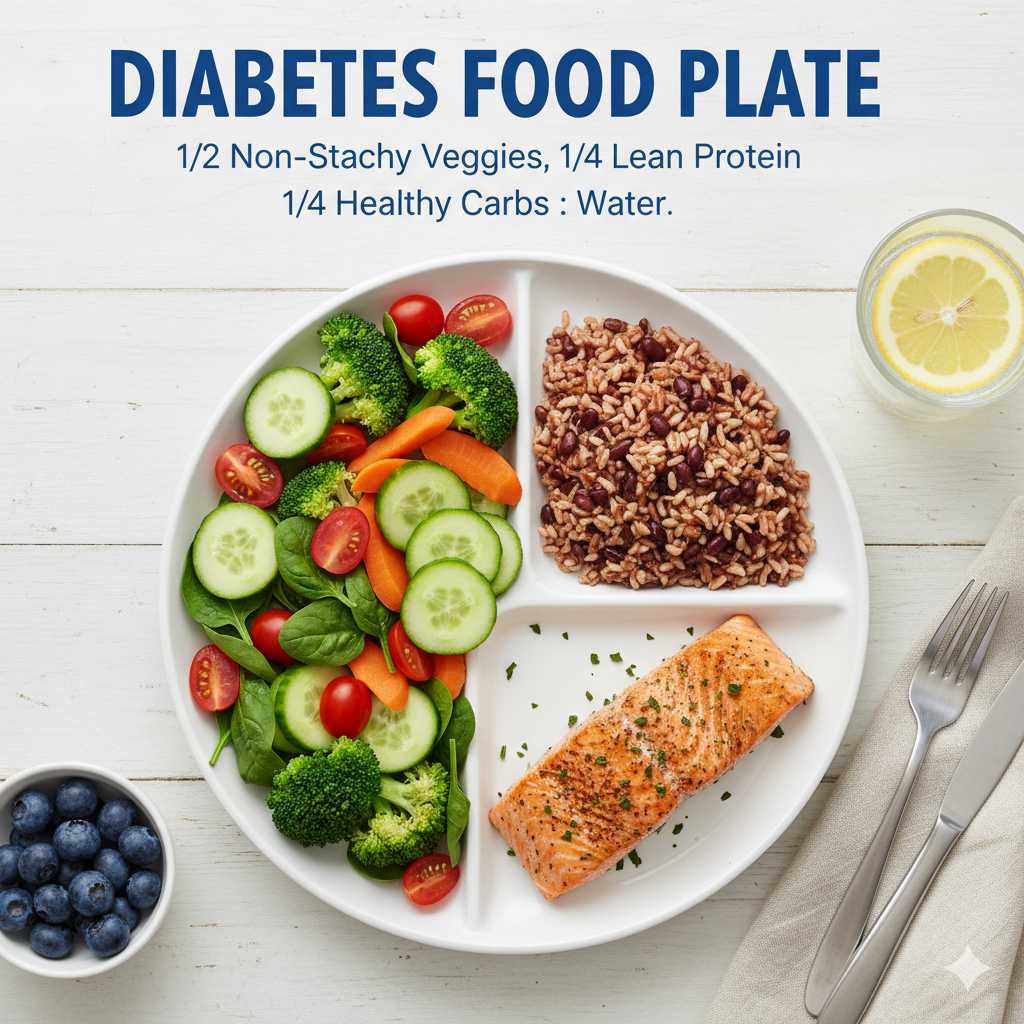
\includegraphics[width=0.75\textwidth]{./plate_figure.png}
  \caption{The Diabetes Plate Method: a visual guide for balanced meals.
  Half the plate is filled with non-starchy vegetables, one quarter with
  lean protein, and one quarter with carbohydrate-containing foods such as
  whole grains, starchy vegetables, or fruit. This simple approach helps
  control carbohydrate intake without requiring precise gram-counting.
  \emph{Source: ADA / adapted from the diabetes food plate concept.}}
  \label{fig:plate}
\end{figure}

Key nutrition principles from the Standards include:

\begin{itemize}
  \item \textbf{Carbohydrate management}: focus on total carbohydrate intake
        rather than the type of sugar alone. Fibre-rich, whole-food sources
        (vegetables, legumes, whole grains) are preferred.
  \item \textbf{Protein}: lean protein sources (poultry, fish, tofu, legumes)
        contribute to satiety and have a minimal direct effect on blood
        glucose.
  \item \textbf{Fat}: emphasis on unsaturated fats (olive oil, nuts,
        avocados) and limitation of saturated and trans fats for
        cardiovascular risk reduction.
  \item \textbf{Portion control}: the Plate Method directly addresses this
        by dividing the plate into visually distinct sections.
\end{itemize}

The Standards recommend that all people with diabetes receive individualised
medical nutrition therapy (MNT) provided by a registered dietitian nutritionist
(Level~A evidence).

\subsection{Weight management and obesity treatment}

Section~8 of the Standards (endorsed by The Obesity Society) addresses
obesity and weight management. For people with type~2 diabetes who are
overweight or have obesity, the Standards recommend:

\begin{itemize}
  \item \textbf{Lifestyle intervention}: moderate calorie reduction (500--750
        kcal/day deficit) combined with at least 150~minutes per week of
        moderate-intensity physical activity.
  \item \textbf{Anti-obesity medications}: when lifestyle alone is
        insufficient, medications such as glucagon-like peptide~1 (GLP-1)
        receptor agonists (e.g., semaglutide, tirzepatide) are recommended
        for chronic weight management (Level~A evidence).
  \item \textbf{Metabolic (bariatric) surgery}: considered for individuals
        with type~2 diabetes and BMI $\geq$~35~kg/m$^2$ who have not
        achieved durable weight loss with non-surgical methods (Level~A
        evidence).
\end{itemize}

\subsection{Pharmacologic management of glucose}

The Standards provide a detailed, evidence-based algorithm for glucose-lowering
medications, stratified by type of diabetes, cardiovascular and kidney
comorbidity, and individual treatment goals.

\subsubsection{Type~1 diabetes}

People with type~1 diabetes require lifelong insulin therapy. The Standards
recommend:

\begin{itemize}
  \item \textbf{Multiple daily injections (MDI)} or \textbf{continuous
        subcutaneous insulin infusion (CSII)} via pump, with AID systems
        preferred where available.
  \item \textbf{Basal-bolus regimens}: a long-acting (basal) insulin
        combined with rapid-acting (bolus) insulin before meals.
  \item \textbf{Individualised glucose targets}: generally fasting/pre-meal
        glucose 80--130~mg/dL and postprandial glucose $<$180~mg/dL,
        adjusted for age, hypoglycaemia risk, and life expectancy.
\end{itemize}

\subsubsection{Type~2 diabetes}

The pharmacologic approach to type~2 diabetes has changed substantially in
recent years. The 2026 Standards reflect a shift from a purely
glucose-centred algorithm to one that prioritises \textbf{cardiovascular and
renal protection}. Key recommendations:

\begin{itemize}
  \item \textbf{First-line therapy}: metformin, unless contraindicated or
        not tolerated (Level~A evidence). For people with established
        atherosclerotic cardiovascular disease (ASCVD), heart failure, or
        chronic kidney disease (CKD), a GLP-1 receptor agonist or an SGLT2
        inhibitor is recommended regardless of baseline HbA1c (Level~A).
  \item \textbf{Second-line agents}: if glycaemic targets are not met,
        options include GLP-1 receptor agonists, SGLT2 inhibitors, DPP-4
        inhibitors, thiazolidinediones, or insulin, chosen based on
        individual patient characteristics, comorbid conditions, and
        treatment goals.
  \item \textbf{Combination therapy}: early combination of agents with
        complementary mechanisms is increasingly favoured to achieve
        durable glycaemic control.
  \item \textbf{Insulin}: when oral agents are insufficient, basal insulin
        is added. The Standards provide detailed guidance on initiation,
        titration, and intensification.
\end{itemize}

\begin{table}[H]
\centering
\small
\caption{Major classes of glucose-lowering medications in the 2026 Standards}
\label{tab:meds}
\begin{tabularx}{\textwidth}{lYY}
\toprule
Medication Class & Key Examples & Primary Considerations \\
\midrule
Metformin & & First-line T2D; low cost, low hypoglycaemia risk;
caution in advanced CKD. \\
GLP-1 receptor agonists & Semaglutide, tirzepatide, dulaglutide & Weight
loss, cardiovascular benefit, renal protection. \\
SGLT2 inhibitors & Empagliflozin, dapagliflozin & Heart failure and CKD
benefit; slight weight loss; risk of genital infections. \\
DPP-4 inhibitors & Sitagliptin, linagliptin & Neutral weight effect; no
cardiovascular benefit beyond safety. \\
Insulin (basal/bolus) & Glargine, degludec, lispro & Most potent glucose
lowering; essential in T1D; risk of hypoglycaemia. \\
\bottomrule
\end{tabularx}
\end{table}

\subsection{Comprehensive risk reduction}

A key message running throughout the Standards is that diabetes care must
address far more than glucose. \textbf{Cardiovascular disease and risk
management} (Section~10, endorsed by the American College of Cardiology)
includes:

\begin{itemize}
  \item Blood pressure targets ($<$130/80~mmHg for most adults).
  \item Lipid management with statin therapy for most people with diabetes
        (Level~A evidence).
  \item Antiplatelet therapy for those with established ASCVD.
\end{itemize}

\textbf{Chronic kidney disease} (Section~11, newly endorsed by the National
Kidney Foundation) is another major priority, with recommendations for annual
albuminuria and eGFR screening, and use of SGLT2 inhibitors and/or GLP-1
receptor agonists for renoprotection.

\section{Putting it all together: from the Standards to the plate}

The document you provided---the ADA \emph{Standards of Care} introduction and
methodology---is the authoritative backbone of modern diabetes care. The
Diabetes Plate image is a practical, patient-facing tool that translates the
nutrition principles of those Standards into a visual framework anyone can
use.

The connection between the two is straightforward:

\begin{itemize}
  \item The \textbf{Standards} provide the \emph{why} (evidence-based
        rationale, targets, medication algorithms, monitoring protocols).
  \item The \textbf{Plate Method} provides the \emph{how} (a simple,
        actionable starting point for daily meal planning).
  \item \textbf{CGM and AID technologies} bridge the gap further by showing
        individuals exactly how their food choices and medication timing
        affect their glucose levels in real time.
\end{itemize}

No single tool works in isolation. The Standards emphasise that effective
diabetes care requires the full care team---clinicians, diabetes educators,
dietitians, behavioural health specialists, and the person with diabetes
themselves---working together with shared goals.

\section{Caveats and next steps}

While this report summarises the core themes, the full ADA Standards of Care
2026 is a comprehensive document spanning 16 sections. The introduction and
methodology reviewed here establishes the rigorous process behind each
recommendation, but the detailed clinical guidance (including specific
medication algorithms, paediatric care, pregnancy management, and
complication screening) resides in the individual sections.

\textbf{Key limitations to keep in mind:}

\begin{itemize}
  \item The Standards are updated annually; recommendations may shift as new
        evidence emerges.
  \item Individual circumstances---comorbidities, age, preferences, access
        to care---may change how recommendations are applied.
  \item The Plate Method is a starting point; some individuals will need
        more precise carbohydrate counting or specialised dietary approaches.
\end{itemize}

\textbf{Suggested next steps for the reader:}

\begin{enumerate}
  \item Discuss your HbA1c target and monitoring plan with your health care
        team.
  \item Ask about CGM if you or your family member uses insulin or
        experiences problematic hypoglycaemia.
  \item Use the Diabetes Plate Method as a simple guide for meal portions,
        then track how different foods affect your glucose.
  \item Review your cardiovascular and kidney risk factors annually at
        minimum.
  \item Explore whether newer medications (GLP-1 receptor agonists, SGLT2
        inhibitors) might offer additional benefits beyond glucose control.
\end{enumerate}

The ADA Standards of Care is not intended to replace clinical judgement; it
is a resource to inform shared decision-making. The plate on your table and
the numbers on your CGM are both part of the same evidence-based picture of
modern diabetes care.

\end{document}